\documentclass[12pt]{article}

% Idioma y codificación
\usepackage[spanish, es-tabla]{babel}       %es-tabla para que se titule "Tabla"
\usepackage[utf8]{inputenc}

% Márgenes
\usepackage[a4paper,top=3cm,bottom=2.5cm,left=3cm,right=3cm]{geometry}

% Comentarios de bloque
\usepackage{verbatim}

% Paquetes de links
\usepackage[hidelinks]{hyperref}    % Permite enlaces
\usepackage{url}                    % redirecciona a la web

% Más opciones para enumeraciones
\usepackage{enumitem}

% Personalizar la portada
\usepackage{titling}


% Paquetes de tablas
\usepackage{multirow}


%------------------------------------------------------------------------

%Paquetes de figuras
\usepackage{caption}
\usepackage{subcaption} % Figuras al lado de otras
\usepackage{float}      % Poner figuras en el sitio indicado H.


% Paquetes de imágenes
\usepackage{graphicx}       % Paquete para añadir imágenes
\usepackage{transparent}    % Para manejar la opacidad de las figuras

% Paquete para usar colores
\usepackage[dvipsnames]{xcolor}
\usepackage{pagecolor}      % Para cambiar el color de la página

% Habilita tamaños de fuente mayores
\usepackage{fix-cm}


%------------------------------------------------------------------------

% Paquetes de matemáticas
\usepackage{mathtools, amsfonts, amssymb, mathrsfs}
\usepackage[makeroom]{cancel}     % Simplificar tachando
\usepackage{polynom}    % Divisiones y Ruffini
\usepackage{units} % Para poner fracciones diagonales con \nicefrac

\usepackage{pgfplots}   %Representar funciones
\pgfplotsset{compat=1.18}  % Versión 1.18

\usepackage{tikz-cd}    % Para usar diagramas de composiciones
\usetikzlibrary{calc}   % Para usar cálculo de coordenadas en tikz

% Paquete para usar el símbolo de grados
\usepackage{gensymb}

%Definición de teoremas, etc.
\usepackage{amsthm}
%\swapnumbers   % Intercambia la posición del texto y de la numeración

\theoremstyle{plain}

\makeatletter
\@ifclassloaded{article}{
  \newtheorem{teo}{Teorema}[section]
}{
  \theoremstyle{definition}
  \newtheorem{teo}{Teorema}[chapter]  % Se resetea en cada chapter
}
\makeatother

\theoremstyle{definition}
\newtheorem{coro}{Corolario}[teo]           % Se resetea en cada teorema
\newtheorem{prop}[teo]{Proposición}         % Usa el mismo contador que teorema
\newtheorem{lema}[teo]{Lema}                % Usa el mismo contador que teorema

\theoremstyle{remark}
\newtheorem*{observacion}{Observación}

\theoremstyle{definition}

\makeatletter
\@ifclassloaded{article}{
  \newtheorem{definicion}{Definición} [section]     % Se resetea en cada chapter
}{
  \newtheorem{definicion}{Definición} [chapter]     % Se resetea en cada chapter
}
\makeatother

\newtheorem*{notacion}{Notación}
\newtheorem*{ejemplo}{Ejemplo}
\newtheorem*{ejercicio*}{Ejercicio}             % No numerado
\newtheorem{ejercicio}{Ejercicio} [section]     % Se resetea en cada section


% Modificar el formato de la numeración del teorema "ejercicio"
\renewcommand{\theejercicio}{%
  \ifnum\value{section}=0 % Si no se ha iniciado ninguna sección
    \arabic{ejercicio}% Solo mostrar el número de ejercicio
  \else
    \thesection.\arabic{ejercicio}% Mostrar número de sección y número de ejercicio
  \fi
}


\renewcommand\qedsymbol{\small{$\blacksquare$}}         % Cambiar símbolo QED
%------------------------------------------------------------------------

% Paquetes para encabezados
\usepackage{fancyhdr}
\pagestyle{fancy}
\fancyhf{}

\newcommand{\helv}{ % Modificación tamaño de letra
\fontfamily{}\fontsize{12}{12}\selectfont}
\setlength{\headheight}{15pt} % Amplía el tamaño del índice


%\usepackage{lastpage}   % Referenciar última pag   \pageref{LastPage}
\fancyfoot[C]{\thepage}

%------------------------------------------------------------------------

% Conseguir que no ponga "Capítulo 1". Sino solo "1."
\makeatletter
\@ifclassloaded{book}{
  \renewcommand{\chaptermark}[1]{\markboth{\thechapter.\ #1}{}} % En el encabezado
    
  \renewcommand{\@makechapterhead}[1]{%
  \vspace*{50\p@}%
  {\parindent \z@ \raggedright \normalfont
    \ifnum \c@secnumdepth >\m@ne
      \huge\bfseries \thechapter.\hspace{1em}\ignorespaces
    \fi
    \interlinepenalty\@M
    \Huge \bfseries #1\par\nobreak
    \vskip 40\p@
  }}
}
\makeatother

%------------------------------------------------------------------------
% Paquetes de cógido
\usepackage{minted}
\renewcommand\listingscaption{Código fuente}

\usepackage{fancyvrb}
% Personaliza el tamaño de los números de línea
\renewcommand{\theFancyVerbLine}{\small\arabic{FancyVerbLine}}

% Estilo para C++
\newminted{cpp}{
    frame=lines,
    framesep=2mm,
    baselinestretch=1.2,
    linenos,
    escapeinside=||
}


\usepackage{listings} % Para incluir código desde un archivo

\renewcommand\lstlistingname{Código Fuente}
\renewcommand\lstlistlistingname{Índice de Códigos Fuente}

% Definir colores
\definecolor{vscodepurple}{rgb}{0.5,0,0.5}
\definecolor{vscodeblue}{rgb}{0,0,0.8}
\definecolor{vscodegreen}{rgb}{0,0.5,0}
\definecolor{vscodegray}{rgb}{0.5,0.5,0.5}
\definecolor{vscodebackground}{rgb}{0.97,0.97,0.97}
\definecolor{vscodelightgray}{rgb}{0.9,0.9,0.9}

% Configuración para el estilo de C similar a VSCode
\lstdefinestyle{vscode_C}{
  backgroundcolor=\color{vscodebackground},
  commentstyle=\color{vscodegreen},
  keywordstyle=\color{vscodeblue},
  numberstyle=\tiny\color{vscodegray},
  stringstyle=\color{vscodepurple},
  basicstyle=\scriptsize\ttfamily,
  breakatwhitespace=false,
  breaklines=true,
  captionpos=b,
  keepspaces=true,
  numbers=left,
  numbersep=5pt,
  showspaces=false,
  showstringspaces=false,
  showtabs=false,
  tabsize=2,
  frame=tb,
  framerule=0pt,
  aboveskip=10pt,
  belowskip=10pt,
  xleftmargin=10pt,
  xrightmargin=10pt,
  framexleftmargin=10pt,
  framexrightmargin=10pt,
  framesep=0pt,
  rulecolor=\color{vscodelightgray},
  backgroundcolor=\color{vscodebackground},
}

%------------------------------------------------------------------------

% Comandos definidos
\newcommand{\bb}[1]{\mathbb{#1}}
\newcommand{\cc}[1]{\mathcal{#1}}

% I prefer the slanted \leq
\let\oldleq\leq % save them in case they're every wanted
\let\oldgeq\geq
\renewcommand{\leq}{\leqslant}
\renewcommand{\geq}{\geqslant}

% Si y solo si
\newcommand{\sii}{\iff}

% Letras griegas
\newcommand{\eps}{\epsilon}
\newcommand{\veps}{\varepsilon}
\newcommand{\lm}{\lambda}

\newcommand{\ol}{\overline}
\newcommand{\ul}{\underline}
\newcommand{\wt}{\widetilde}
\newcommand{\wh}{\widehat}

\let\oldvec\vec
\renewcommand{\vec}{\overrightarrow}

% Derivadas parciales
\newcommand{\del}[2]{\frac{\partial #1}{\partial #2}}
\newcommand{\Del}[3]{\frac{\partial^{#1} #2}{\partial^{#1} #3}}
\newcommand{\deld}[2]{\dfrac{\partial #1}{\partial #2}}
\newcommand{\Deld}[3]{\dfrac{\partial^{#1} #2}{\partial^{#1} #3}}


\newcommand{\AstIg}{\stackrel{(\ast)}{=}}
\newcommand{\Hop}{\stackrel{L'H\hat{o}pital}{=}}

\newcommand{\red}[1]{{\color{red}#1}} % Para integrales, destacar los cambios.

% Método de integración
\newcommand{\MetInt}[2]{
    \left[\begin{array}{c}
        #1 \\ #2
    \end{array}\right]
}

% Declarar aplicaciones
% 1. Nombre aplicación
% 2. Dominio
% 3. Codominio
% 4. Variable
% 5. Imagen de la variable
\newcommand{\Func}[5]{
    \begin{equation*}
        \begin{array}{rrll}
            #1:& #2 & \longrightarrow & #3\\
               & #4 & \longmapsto & #5
        \end{array}
    \end{equation*}
}

%------------------------------------------------------------------------
\setlength{\parindent}{0pt} % quitar la sangría

\setlist[itemize, 1]{label=\textbullet \textbf{)}}  % Cambiar las viñetas a círculos

\def\endsquare{%
  \begin{flushright}
      \small{$\blacksquare$}
  \end{flushright}
}

\newcommand{\apuntar}[1]{%
  \hyperlink{#1}{\textbf{(#1)}}%p
}

\newcommand{\objetivo}[1]{%
  \textbf{(\hypertarget{#1}{#1})}
}


\usepackage{xkeyval} % Para el paso de argumentos

\usepackage{graphicx}

% Definir la carpeta de las imágenes
\graphicspath{{../_assets}{../../_assets}{../../../_assets}}

% Definir el comando \portada
\makeatletter
\define@key{portada}{titulo}{\def\titulo{#1}}
\define@key{portada}{subtitulo}{\def\subtitulo{#1}}
\define@key{portada}{autor}{\def\autor{#1}}
\define@key{portada}{año}{\def\año{#1}}
\define@key{portada}{color página}{\def\colorpagina{#1}}
\define@key{portada}{imagen}{\def\imagen{#1}}

\newcommand*{\portada}[1][]{%
  % Encabezado
  \fancyhead[L]{\helv \titulo}
  \fancyhead[R]{\helv \nouppercase{\leftmark}}

    % Definimos las claves y sus valores por defecto
  \setkeys{portada}{%
    titulo=Sin Título,%
    subtitulo=Sin Subtítulo,%
    autor=Autor Desconocido,%
    año=Sin Año,%
    color página=white,%
    imagen=Logo-UGR-Black.png, #1}%
    \begin{titlepage}
        \centering
        \pagecolor{\colorpagina} % Cambia el color de fondo de la portada
        {\includegraphics[width=0.2\textwidth]{\imagen}\par}
        \vspace{1cm}
        {\bfseries\LARGE Universidad de Granada \par}
        \vspace{1cm}
        {\scshape\Large Doble Grado en Ingeniería Informática y Matemáticas \par}
        \vspace{3cm}
        {\scshape\Huge \titulo \par}
        \vspace{3cm}
        {\itshape\Large \subtitulo \par}
        \vfill
        {\Large Autor: \par}
        {\Large \autor \par}
        \vfill
        {\Large \año \par}
    \end{titlepage}%
    \pagecolor{white}
}
\usepackage{ wasysym }

\definecolor{bgcolor}{rgb}{0.95, 0.95, 0.95} % Gris claro
\setminted{bgcolor=bgcolor,fontsize=\footnotesize} % Configuración global

\begin{document}

\portada[%
        titulo=Modelos de Computación,
        subtitulo=Práctica Lex/Flex,
        autor=Jesús Muñoz Velasco\\Daniel Morán Sánchez,
        año=Curso 2024-2025,
        imagen=../../../../documents/_assets/Logo-UGR-Black.png]

\tableofcontents

\newpage

\section{Introducción}

El objetivo principal de esta práctica es la de resolver una traducción simple de un código en HTML a pdf utilizando \LaTeX como lenguaje para realizar dicha transformación. Para ello se han seleccionado una serie de estructuras de HTML para transformarlas a su correspondiente código en \LaTeX.\\

En esta implementación, para no complicar demasiado la traducción no se han tenido en cuenta el uso de estilos ni de bloques de código (ya que estos no serían implementables).

\section{Estructuras}
Las principales estructuras de HTML que se han procesado con el programa realizado han sido los siguientes:

\subsection{Bold/Black}
Estas etiquetas HTML ponen en negrita el texto que encierran. Un ejemplo de su uso en un documento HTML sería el siguiente:
\begin{minted}{html}
Esto es una palabra en <strong>negrita</strong> y esta <b>otra</b>.
\end{minted}
Las expresiones regulares que se han utilizado para la detección de estas etiquetas han sido:
\begin{minted}[bgcolor=bgcolor]{python3}
    BOLD    \<strong\>[^\<]*\<\/strong\>
    BLACK    \<b\>[^\<]*\<\/b\>
\end{minted}
De esta forma se reconocerían las etiquetas principales y el texto que encierran, el cual no puede contener el caracter \verb|'<'|. Seguiría un diagrama similar al siguiente:

\begin{center}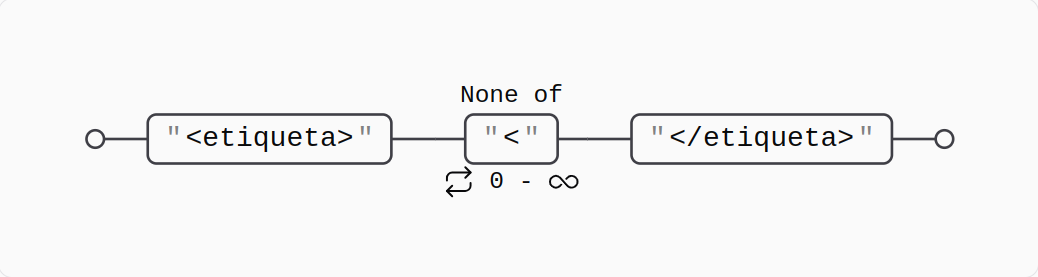
\includegraphics[width=12cm]{./images/image1.png}\end{center}

Donde \verb|'etiqueta'| se cambiará por el nombre de la etiqueta en cada caso. Esta estructura se usará para el resto de etiquetas con un formato similar (ya que es propio de HTML) y por eso no se volverá a desarrollar.\\

Para su traducción a \LaTeX se ha utilizado el entorno \verb|textbf| el cual tiene el mismo resultado en este lenguaje. El ejemplo anterior traducido sería el siguiente:
\begin{minted}{latex}
Esto es una palabra en \textbf{negrita} y esta \textbf{otra}.
\end{minted}
% Para ello se ha utilizado el siguiente código en \verb|c++|:
% \begin{minted}{cpp}
% {BOLD}  {
%     string tmp = yytext;
%     /* Procesa el contenido entre <strong> y </strong> */
%     resultado += "\\textbf{" 
%                + cadena_entre("<strong>", "</strong>", yytext) + "}";
% }

% {BLACK}  {
%     string tmp = yytext;
%     /* Procesa el contenido entre <b> y </b> */
%     resultado += "\\textbf{" + cadena_entre("<b>", "</b>", yytext) + "}";
% }
% \end{minted}

\subsection{Italic}
Esta etiqueta hace referencia al texto en cursiva. Sigue la misma estructura que antes. Un ejemplo de su uso en un documento HTML sería el siguiente:
\begin{minted}{html}
Esto es una palabra en <em>cursiva</em>.
\end{minted}
La expresión regular utilizada para su reconocimiento ha sido la siguiente:
\begin{minted}{python3}
    ITALIC    \<em\>[^\<]*\<\/em\>
\end{minted}
Su traducción a \LaTeX se ha implementado mediante el entorno \verb|textit|. El ejemplo anterior traducido sería el siguiente:
\begin{minted}{latex}
Esto es una palabra en \texit{cursiva}.
\end{minted}

\subsection{Underlined}
Esta etiqueta se usa para el texto subrayado. Un ejemplo de su uso en HTML sería el siguiente:
\begin{minted}{html}
Esto es una palabra <u>subrayada</u>.
\end{minted}
De nuevo, la expresión regular con la estructura de etiquetas sería la siguiente:
\begin{minted}{python3}
    UNDERLINED    \<u\>[^\<]*\<\/u\>
\end{minted}
La implementación del subrayado se ha realizado en \LaTeX mediante \verb|underline|. El ejemplo anterior quedaría de la siguiente forma:
\begin{minted}{latex}
Esto es una palabra \underline{subrayada}.
\end{minted}

\subsection{Section, Subsection y Subsubsection}
Estas etiquetas se utilizan para delimitar secciones, permitiendo usar una jerarquía. En HTML se implementan con las etiquetas \verb|h1,...,h6|. En \LaTeX solo se permiten 3 niveles de jerarquía por lo que solo se han implementado \verb|h1|, \verb|h2| y \verb|h3|. Con el resto de etiquetas se podría hacer algún tipo de gestión pero como dependería de la implementación deseada no se ha realizado ninguna. Un ejemplo del uso de estas etiquetas en un documento HTML sería el siguiente:
\begin{minted}{html}
<h1>Esto es un título</h1>
<h2>Esto es un subtítulo</h2>
<h3>Esto es un subsubtítulo</h3>
\end{minted}
Las expresiones regulares utilizadas para su detección han sido:
\begin{minted}{python3}
    SECTION    \<h1\>[^\<]*\<\/h1\>
    SUBSECTION    \<h2\>[^\<]*\<\/h2\>
    SUBSUBSECTION    \<h3\>[^\<]*\<\/h3\>
\end{minted}
Si se quisiera agrupar \verb|h3,...,h6|, se podría modificar esta última expresión a
\begin{minted}{python3}
    SUBSUBSECTION    \<h[3-6]\>[^\<]*\<\/h[3-6]\>
\end{minted}
Aunque no garantizaría la corrección del código, es decir, no tendría por qué coincidir la etiqueta de apertura con la de cierre (podría admitir cadenas como por ejemplo \verb|<h4>subsubtitulo</h5>|). \\

La traducción de estas etiquetas a \LaTeX se ha realizado mediante \verb|section|, \verb|subsection| y \verb|subsubsection| respectivamente. El ejemplo anterior quedaría de la siguiente forma:
\begin{minted}{latex}
\section{Esto es un título}
\subsection{Esto es un subtítulo}
\subsubsection{Esto es un subsubtítulo}
\end{minted}

\subsection{Paragraph}
Esta estructura se utiliza para delimitar párrafos en HTML. Un ejemplo de su uso en HTML sería el siguiente:
\begin{minted}{html}
<p>Esto es un párrafo.</p>
\end{minted}
La expresión regular utilizada ha sido la siguiente:
\begin{minted}{python3}
    PARAGRAPH    \<p\>[^\<]*\<\/p\>
\end{minted}
Su traducción se ha realizado simplemente añadiendo el texto sin ningún entorno ya que \LaTeX es un lenguaje de procesamiento de texto y todo el texto sin etiqueta se interpreta como párrafo. De esta forma el ejemplo anterior traducido quedaría
\begin{minted}{latex}
Esto es un párrafo.
\end{minted}

\subsection{Image}
En HTML se utiliza la etiqueta \verb|img| para insertar imágenes en el documento. En este caso sí se ha admitido algún parámetro adicional como el tamaño de la imagen (se ha considerado opcional). Un ejemplo de su uso en HTML sería el siguiente:
\begin{minted}{html}
<img src="image.png" width="300" height="200">
\end{minted}
Esto indica que la dirección de la imagen es \verb|image.png| y que tiene unas dimensiones de \verb|300 x 200 px|. Los parámetros relativos al tamaño son opcionales (pueden incluirse ambos, uno o ninguno y seguirá funcionando correctamente). De este modo, la expresión regular utilizada ha sido la siguiente:
\begin{minted}{python3}
    IMG    \<img.*src=\"[^\"]*\".*\>
\end{minted}
Lo cual admite las cadenas que empiecen por \verb|<img|, que sigan por cualquier cadena de caracteres (\verb|.*|), después tienen que contener la cadena \verb|src="| seguida de cualquier cadena que no incluya el caracter \verb|"| y que se cierre con dicho caracter. Después vuelve a admitir cualquier cadena hasta que se cierre con \verb|>|. Podemos verlo gráficamente con el siguiente diagrama:

\begin{center}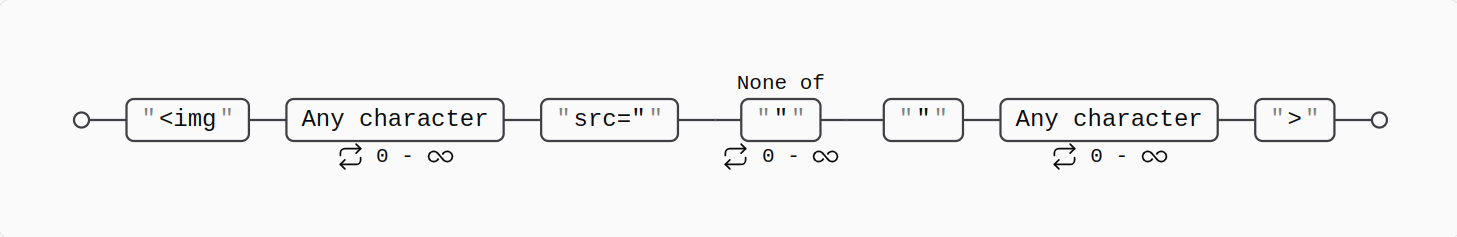
\includegraphics[width=15cm]{./images/image2.png}\end{center}

Su traducción a \LaTeX se ha realizado mediante \verb|includegraphics| el cual admite parámetros opcionales, facilitando su adaptación. El ejemplo anterior quedaría de la siguiente forma:
\begin{minted}{latex}
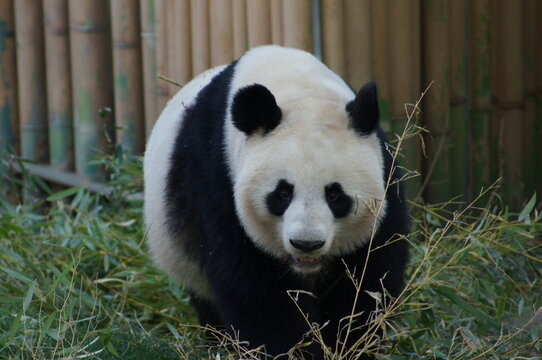
\includegraphics[width=300px, height=200px]{image.png}
\end{minted}

\subsection{Link}
La estructura con etiqueta \verb|a| permite en HTML insertar hiperenlaces a otras páginas. Su sintáxis incluye un parámetro \verb|href| donde se indica la dirección de la página enlazada. Un ejemplo de su uso en un documento HTML sería el siguiente:
\begin{minted}{html}
<a href="https://ejemplo.com">Esto es un enlace</a>
\end{minted}
Sabiendo esto, la expresión regular empleada ha sido la siguiente:
\begin{minted}{python3}
    LINK    \<a\ href=\"[^\"]*\"\>[^\<]*\<\/a\>
\end{minted}
Como se puede ver sigue una estructura mixta entre la de etiquetas (con la etiqueta \verb|a| para cierre y apertura) y la de parámetros vista para imágenes. Su estructura se podría representar de la siguiente forma.

\begin{center}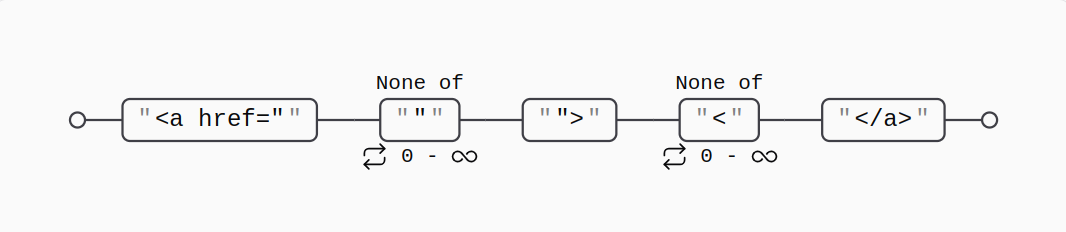
\includegraphics[width=15cm]{./images/image3.png}\end{center}

Para su implementación en \LaTeX se ha empleado el comando \verb|href| el cual admite tanto el enlace como el texto que se mostrará. El ejemplo anterior adaptado se verá de la siguiente forma:
\begin{minted}{latex}
\href{https://ejemplo.com"}{Esto es un enlace}
\end{minted}

\subsection{Newline}
En  HTML existe una etiqueta especial, \verb|br| (break) que inserta un salto de línea. No requiere de una etiqueta de cierre y se podría usar de la siguiente forma.
\begin{minted}{html}
Esto es una línea con salto al final.<br>
\end{minted}
Su expresión regular es bastante simple ya que consiste en la detección literal de esta cadena.
\begin{minted}{python3}
    NEWLINE \<br\>
\end{minted}
Su adaptación a \LaTeX se ha implementado con el doble escape, \verb|\\| el cual tiene un efecto similar. El ejemplo anterior quedaría de la siguiente forma:
\begin{minted}{latex}
Esto es una línea con salto al final.\\
\end{minted}

\subsection{Unordered List}
Esta estructura se utiliza en HTML para crear listas no ordenadas, es decir, cuyos elementos se encuentrar indentados por viñetas (no números). Su sintáxis en HTML consiste en una etiquetación (\verb|ul|) para delimitar la lista y otra (\verb|li|) para delimitar cada elemento de la lista. Una lista puede contener tantos elementos como se requiera. Un ejemplo de su uso en HTML sería el siguiente:
\begin{minted}{html}
<ul>
    <li>Esto</li>
    <li>Es una lista</li>
    <li>No ordenada</li>
</ul>
\end{minted}
Su expresión regular ha resultado en:
\begin{minted}{python3}
    ULIST    \<ul\>(\n|\ |\t)*(\<li\>[^\<]*\<\/li\>(\n|\ |\t)*)*\<\/ul\>
\end{minted}
Lo cual tiene en cuenta la estructura que se ha mencionado anteriormente además de considerar los espacios en blanco, tabulaciones y saltos de línea (\verb|\n|$|$\verb|\ |$|$\verb|\t|) que pueda haber entre las etiquetas. El diagrama resultante de esta expresión regular sería el siguiente:

\begin{center}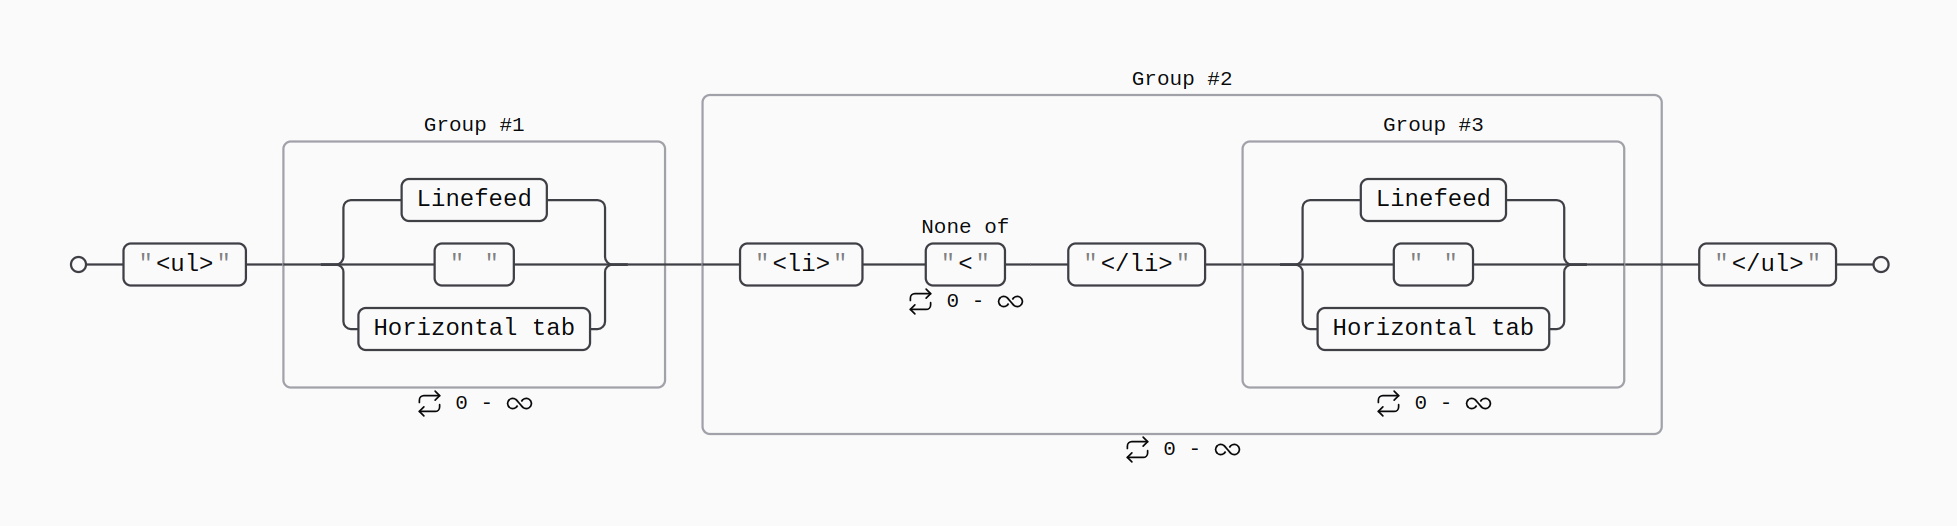
\includegraphics[width=15cm]{./images/image4.png}\end{center}

Su traducción a \LaTeX se ha implementado utilizando el entorno \verb|itemize|, en el que los elementos están delimitados por el comando \verb|item|. De esta forma, el ejemplo anterior quedaría de la siguiente forma:
\begin{minted}{latex}
\begin{itemize}
    \item Esto
    \item Es una lista
    \item No ordenada
\end{itemize}
\end{minted}

\subsection{Ordered List}
Esta estructura es muy similar a la anterior y se utiliza en HTML para crear listas ordenadas, es decir, cuyos elementos están numerados. Su sintáxis es idéntica a la anterior a excepción de que la etiqueta que delimita la lista será \verb|ol| en lugar de \verb|ul|. Un ejemplo de su uso en HTML sería el siguiente:
\begin{minted}{html}
<ol>
    <li>Esto</li>
    <li>Es una lista</li>
    <li>Ordenada</li>
</ol>
\end{minted}
Aálogamente, su expresión regular será 
\begin{minted}{python3}
    OLIST    \<ol\>(\n|\ |\t)*(\<li\>[^\<]*\<\/li\>(\n|\ |\t)*)*\<\/ol\>
\end{minted}
Que no se desarrollará por ser igual a la anterior pero con el cambio ya explicado. Su implementación a \LaTeX se ha realizado con el entorno \verb|enumerate| el cual funciona exactamente igual que \verb|itemize| pero numerando los items. Por tanto, el ejemplo anterior quedaría de la siguiente forma:
\begin{minted}{latex}
\begin{enumerate}
    \item Esto
    \item Es una lista
    \item Ordenada
\end{enumerate}
\end{minted}

\subsection{Table}
La creación de tablas en HTML sigue una estructura algo compleja y se realiza a varios niveles. En primer lugar, una etiqueta \verb|table| delimita por completo a la tabla. Cada fila de la tabla estará delimitada por la etiqueta \verb|tr| (table row). Por último, cada celda dentro de cada fila podrá estar delimitada por las etiquetas \verb|th| (cabecera) o \verb|td|. De esta forma, un ejemplo de tabla con 3 columnas y 2 filas (siendo la primera la cabecera) que se podría hacer en HTML sería la siguiente:
\begin{minted}{html}
<table>
    <tr>
        <th>Esto</th>
        <th>Es la</th>
        <th>Cabecera</th>
    </tr>
    <tr>
        <td>Esto</td>
        <td>Es el resto</td>
        <td>de la tabla</td>
    </tr>
</table>
\end{minted}
Su expresión regular utiliza la misma estrategia usada para las listas de gestión de espacios en blanco y por ello resulta un poco compleja de leer aunque con el diagrama que la representa se entenderá mejor. Se ha considerado la siguiente expresión (sin el salto de línea, que se ha puesto para su correcta visualización en este documento).
\begin{minted}{python3}
    TABLE    \<table\>(\n|\ |\t)*(\<tr\>((\n|\ |\t)*(\<td\>[^\<]*\<\/td>|\<th\>
             [^\<]*\<\/th>)(\n|\ |\t)*)*\<\/tr\>(\n|\ |\t)*)*<\/table\>
\end{minted}
El diagrama que resulta es el siguiente (se recomienda hacer un poco de zoom para verlo mejor):

\begin{center}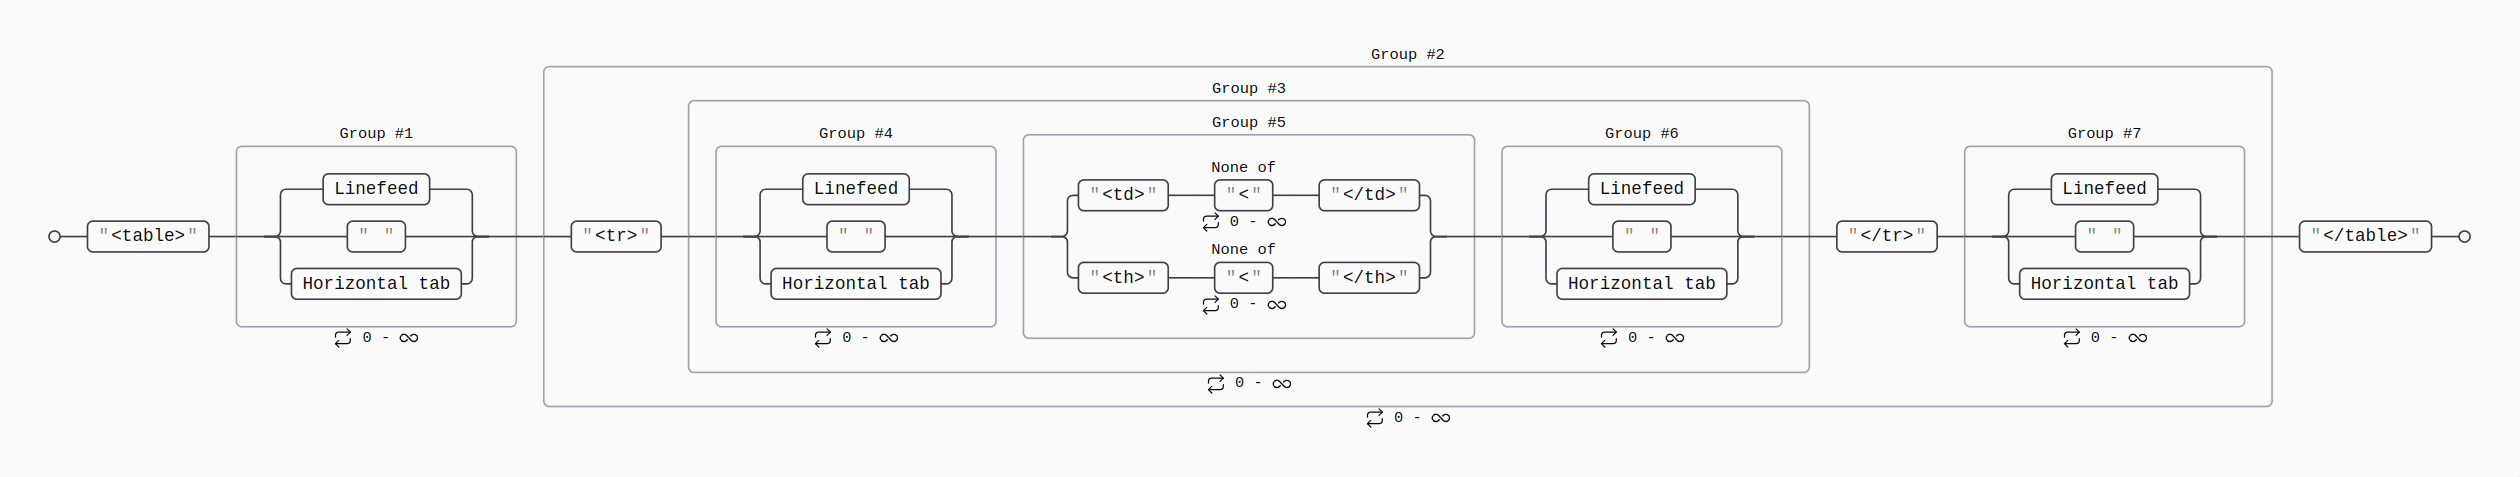
\includegraphics[width=15cm]{./images/image5.png}\end{center}

Su traducción a \LaTeX se ha realizado mediante el entorno \verb|tabular| en el cual se ha implementado un código en \verb|c++| que permite tablas dinámicas, es decir, de cualquier numero de columnas (ya que en \LaTeX se debe saber a priori). Esto se hace contando primero el número de elementos de la primera fila y asumiendo que el resto de la tabla tendrá dicho número de columnas. En \LaTeX cada fila se representará como una línea acabada por salto de línea (\verb|\\|) y las celdas se separarán horizontalmente con el separador \verb|&|. Además, para las filas de encabezado (con etiqueta \verb|th|) se ha insertado el texto en un entorno \verb|strong|. Además se han añadido todos los bordes de la tabla (esto se podría cambiar pero se ha decidido que es lo que mejor representa una tabla). Para ello, entre cada fila y al principio y al final de la tabla se inserta el comando \verb|hline| que añade los separadores horizontales. Los separadores verticales se especifican en las dimensiones de la tabla .De esta forma, la tabla anterior quedaría de la siguiente forma:
\begin{minted}{latex}
\begin{tabular}{|c|c|c|}
    \hline
    \textbf{Esto} & \textbf{Es la} & \textbf{Cabecera} \\
    \hline
    Esto & Es el resto & de la tabla \\
    \hline
\end{tabular} 
\end{minted}

\subsection{Head}
En HTML un documento se estructura en varias partes (estructura general del documento). Una de ellas es el \verb|head| en el cual se especifican configuraciones varias como palabras claves para la búsqueda, idioma, enlaces a hojas de estilo, etc. Las configuraciones que nos interesan por poder ser pasadas a \LaTeX son únicamente el título (con etiqueta \verb|title|) y el autor (con etiqueta \verb|author|). Esta sección en su totalidad está delimitada por la etiqueta \verb|head|. De esta forma, un ejemplo de head de un documento HTML sería la siguiente:
\begin{minted}{html}
<head>
    <meta charset="UTF-8">
    <meta name="viewport" content="width=device-width, initial-scale=1.0">
    <title>Document</title>
    <meta name="author" content="Jesús y Dani">
    <style>
        table, th, td{
            border: 1px solid black;
            border-collapse: collapse;
        };
    </style>
</head>
\end{minted}
Como puede contener cualquier etiqueta en su interior, la expresión regular utilizada ha sido mucho más general que las utilizadas hasta ahora resultando en 
\begin{minted}{python3}
    \<head\>((.|\n)*?)\<\/head\>
\end{minted}
Lo cual admite cualquier caracter incluyendo saltos de línea. De esta sección solo nos interesa detectar el autor y el título, lo cual se ha implementado en \verb|c++| sin utilizar las utilidades de \verb|flex| (por lo admitir realizar búsquedas recursivas y por la necesidad de eliminar el resto del contenido por ser inútil y causar fallos en la compilación del archivo \LaTeX de salida). Por tanto, la adaptación a \LaTeX del ejemplo anterior sería únicamente lo siguiente:
\begin{minted}{latex}
\title{Document}
\author{Jesús y Dani}
\end{minted}

\subsection{Body}
Al igual que la sección anterior, otra parte básica de la estructura general de un HTML es \verb|body|. En él se incluyen los elementos que se visualizarán al procesar un archivo HTML. Está encerrado por la etiqueta \verb|body| y en su interior se incluyen el resto de estructuras que se han mencionado hasta el momento. Es por ello que se hace de forma ligeramente distinta a los demás. Un ejemplo de uso de esta estructura en un documento HTML sería el siguiente:
\begin{minted}{html}
<body>
    Esto es el cuerpo del documento.
</body>
\end{minted}
Su expresión regular se ha trabajado de forma distinta ya que se va a emplear una sustitución literal. Se ha propuesto las siguientes expresiones:
\begin{minted}{python3}
    BODY_BEGIN    \<body\>
    BODY_END    \<\/body\>
\end{minted}
De esta forma se buscan literalmente las etiquetas sin interferir lo que encierran y se han traducido a \LaTeX utilizando la apertura y clausura del entorno \verb|document| respectivamente. Así, el ejemplo anterior quedaría de la siguiente forma:
\begin{minted}{latex}
\begin{document}
    Esto es el cuerpo del documento.
\end{document}
\end{minted}
Cabe destacar que esta estrategia se podría haber usado en otros casos y hubiese permitido la anidación de varias estructuras pero se ha decidido no hacerlo así para poder buscar expresiones regulares más complejas y que no fuesen literales.

\subsection{Ignore}
Por la naturaleza de los archivos HTML se incluyen campos que deben ser eliminados para la correcta compilación del archivo de salida en formato \verb|tex|. Es por esto que se ha decidido ignorar (no pasar al documento final) las estructuras que se adecúen a la siguiente expresión regular:
\begin{minted}{python3}
    IGNORE  (\<!DOCTYPE\ html\>|\<html\ lang=\"[^\"]*\"\>|\<\/html>)
\end{minted}
Con esto se consigue pasar finalmente a un documento \LaTeX con una sintáxis correcta. Estos campos que se ignoran son
\begin{itemize}
    \item El indicador de que es un archivo HTML (\verb|<!DOCTYPE html>|).
    \item La apertura de la etiqueta \verb|html| que incluye \verb|head| y \verb|body| y que por tanto no tiene por qué pasar al documento final de ninguna forma especial, sino procesando como ya se ha mencionado las estructuras que contiene.
    \item El cierre de la etiqueta \verb|html|.
\end{itemize}

\section{Ejemplo de uso}

Para probar el programa se ha realizado un documento HTML genérico llamado \verb|fichero.html| que incluye todas las estructuras que se han trabajado en esta práctica para ver su correcto funcionamiento. El documento HTML contiene lo siguiente:

\begin{minted}{html}
<!DOCTYPE html>
<html lang="en">
<head>
    <meta charset="UTF-8">
    <meta name="viewport" content="width=device-width, initial-scale=1.0">
    <title>Document</title>
    <meta name="author" content="Jesús y Dani">
    <style>
        table, th, td{
            border: 1px solid black;
            border-collapse: collapse;
        };
    </style>
</head>
<body>

<h1>Esto es un título</h1>
<h2>Esto es un subtítulo</h2>
<h3>Esto es un subsubtítulo</h3>

Aquí comienza un texto que puede contener palabras en <strong>negrita</strong>, 
en <em>cursiva</em> y <u>subrayadas</u>. 
Puede contener también <a href="https://ejemplo.com">enlaces</a>.
Además, se pueden empezar párrafos como el siguiente:

<p>Esto es un párrafo de un documento HTML que termina con un salto de línea.
</p><br>
Se pueden ver también imágenes como la siguiente:<br>

<img src="image.png" width="300" height="200"><br>

Además se incluye una lista no ordenada:
<ul>
    <li>Esto</li>
    <li>Es una lista</li>
    <li>No ordenada</li>
</ul>

Y una lista ordenada
<ol>
    <li>Esto</li>
    <li>Es una lista</li>
    <li>Ordenada</li>
</ol>

Se añade también una tabla con 3 columnas y cabecera

<table>
    <tr>
        <th>Esto</th>
        <th>Es la</th>
        <th>Cabecera</th>
    </tr>
    <tr>
        <td>Esto</td>
        <td>Es el resto</td>
        <td>de la tabla</td>
    </tr>
</table>

Se añade también una tabla con 2 columnas y sin cabecera 

<table>
    <tr>
        <td>Esto es</td>
        <td>otra tabla</td>
    </tr>
    <tr>
        <td>Esto</td>
        <td>Es el resto</td>
    </tr>
</table>


</body>
</html>
\end{minted}

Al visualizar este código HTML obtendríamos lo siguiente:

\begin{center}\fbox{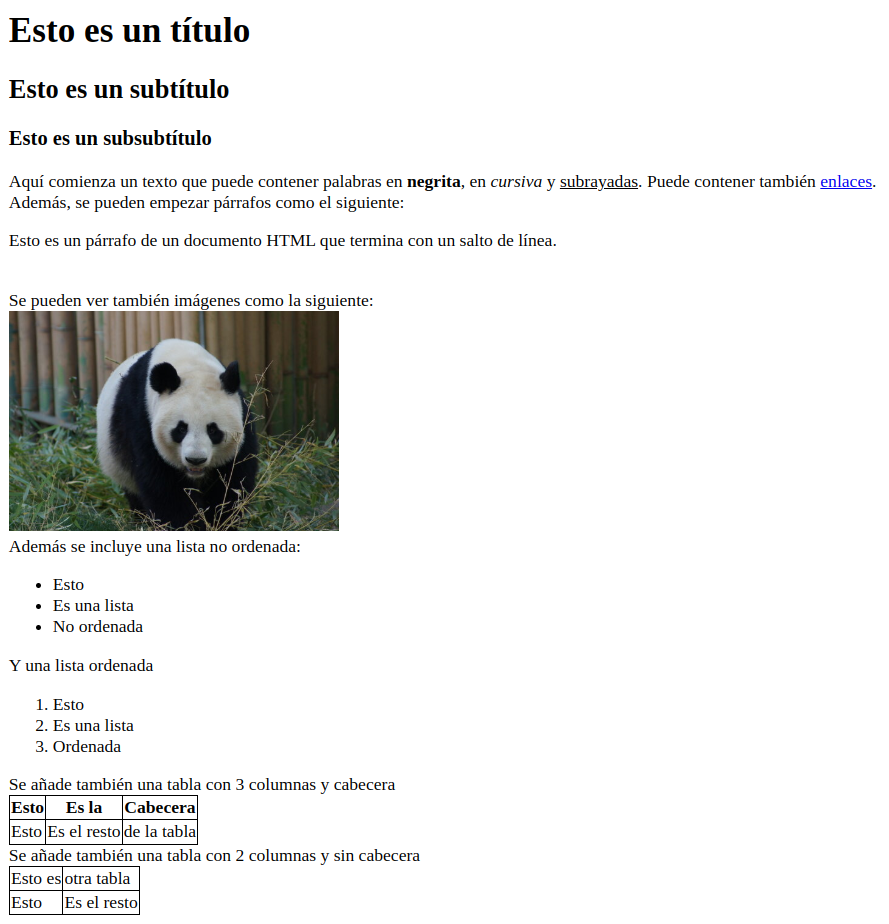
\includegraphics[width=15cm]{./images/image6.png}}\end{center}

Una vez realizado, podemos compilar el programa \verb|html-to-latex.l| de la siguiente forma:
\begin{minted}{bash}
$ flex++ -o ./html-to-latex.yy.cc ./html-to-latex.l
$ g++ -o ./html-to-latex ./html-to-latex.yy.cc
$ ./html-to-latex ./fichero.html > ./salida.tex
$ pdflatex ./salida.tex
\end{minted}

De esta forma se compila el archivo \verb|flex| y se ejecuta sobre \verb|fichero.html| dirigiendo la salida a un documento \verb|salida.tex| que se compila para crear el pdf que se llamará \verb|salida.pdf|. El documento \verb|salida.tex| contendrá lo siguiente:
\begin{minted}{latex}
\documentclass[12pt]{article}
\usepackage{graphicx}
\usepackage{hyperref}


\title{Document}
\author{Jesús y Dani}

\begin{document}


\section{Esto es un título}
\subsection{Esto es un subtítulo}
\subsubsection{Esto es un subsubtítulo}

Aquí comienza un texto que puede contener palabras en \textbf{negrita}, 
en \textit{cursiva} y \underline{subrayadas}. 
Puede contener también \href{https://ejemplo.com"}{enlaces}.
Además, se pueden empezar párrafos como el siguiente:

Esto es un párrafo de un documento HTML que termina con un salto de línea.\\

Se pueden ver también imágenes como la siguiente:\\


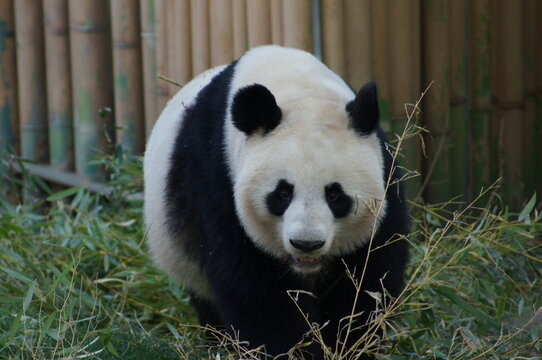
\includegraphics[width=300px, height=200px]{image.png}

Además se incluye una lista no ordenada:
\begin{itemize}
    \item Esto
    \item Es una lista
    \item No ordenada
\end{itemize}


Y una lista ordenada
\begin{enumerate}
    \item Esto
    \item Es una lista
    \item Ordenada
\end{enumerate}


Se añade también una tabla con 3 columnas y cabecera

\begin{tabular}{|c|c|c|}
    \hline
    \textbf{Esto} & \textbf{Es la} & \textbf{Cabecera} \\
    \hline
    Esto & Es el resto & de la tabla \\
    \hline
\end{tabular}


Se añade también una tabla con 2 columnas y sin cabecera 

\begin{tabular}{|c|c|}
    \hline
    Esto es & otra tabla \\
    \hline
    Esto & Es el resto \\
    \hline
\end{tabular}



\end{document}
    
    
    
\end{minted}
Y el pdf resultante se vería de la siguiente forma:\\

\begin{tabular}{cc}
    \fbox{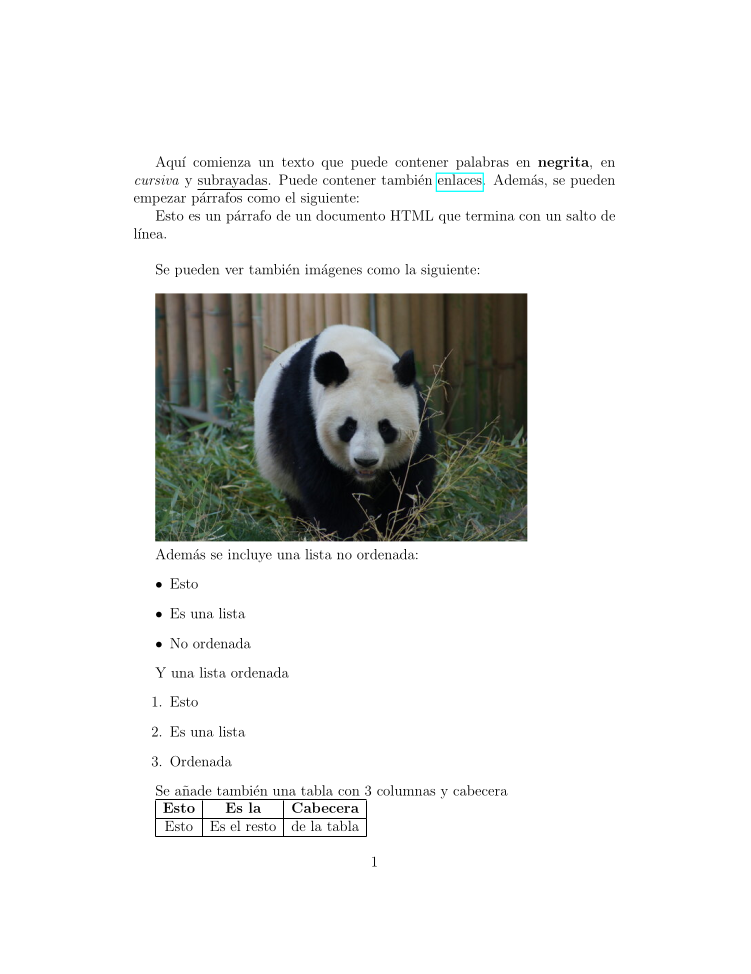
\includegraphics[width=7.5cm]{./images/image7.png}} & 
    \fbox{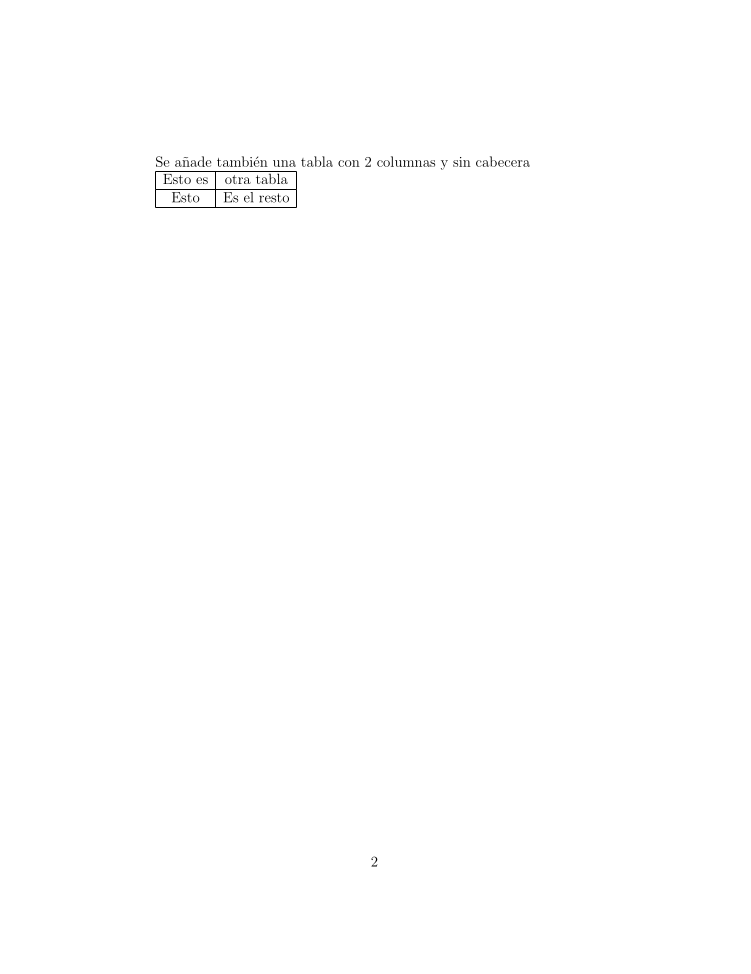
\includegraphics[width=7.5cm]{./images/image8.png}}\\
\end{tabular}
\end{document}